% !TeX root = RJwrapper.tex
\title{Containers and R---the Rockerverse and beyond}
\author{by Daniel Nüst, Robrecht Cannoodt, Dirk Eddelbuettel, Mark Edmondson, Colin Fay, Karthik Ram, Noam Ross, Nan Xiao, Lori Shepherd, Nitesh Turaga, Jacqueline Nolis, Heather Nolis, Hong Ooi, Ellis Hughes, Sean Lopp, Ben Marwick}

\maketitle

\abstract{%
The Rocker project provides widely-used Docker images for R across
different application scenarios. This articles surveys downstream
projects building upon Rocker and presents the current state of R
packages for managing Docker images and controlling containers. We also
look beyond Rocker to other projects connecting containerisation with R,
namely alternative suites of images. These use cases and the variety of
applications demonstrate the power of Rocker specifically and
containerisation in general. We identified common themes across this
diversity: reproducible environments, scalability and effectivity, and
portability across clouds.
}

\hypertarget{introduction}{%
\section{Introduction}\label{introduction}}

\label{intro}

The R community keeps growing. This can be seen in the number of new
packages on CRAN, which keeps on growing exponentially
\citep{cran:2019}, but also in the numbers of conferences, open
educational resources, meetups, unconferences, and companies taking up,
as exemplified by the useR! conference
series\footnote{\href{https://www.r-project.org/conferences/}{https://www.r-project.org/conferences/}},
the global growth of the R and R-Ladies user
groups\footnote{\href{https://www.r-consortium.org/blog/2019/09/09/r-community-explorer-r-user-groups}{https://www.r-consortium.org/blog/2019/09/09/r-community-explorer-r-user-groups}, \href{https://www.r-consortium.org/blog/2019/08/12/r-community-explorer}{https://www.r-consortium.org/blog/2019/08/12/r-community-explorer}},
or the foundation and impact of the
R~Consortium\footnote{\href{https://www.r-consortium.org/news/announcements}{https://www.r-consortium.org/news/announcements}, \href{https://www.r-consortium.org/blog/2019/11/14/data-driven-tracking-and-discovery-of-r-consortium-activities}{https://www.r-consortium.org/blog/2019/11/14/data-driven-tracking-and-discovery-of-r-consortium-activities}}.
All this cements the role of R as the \emph{lingua~franca} of
statistics, data visualisation, and computational research. Coinciding
with the rise of R was the advent of
\href{https://en.wikipedia.org/wiki/Docker_(software)}{Docker} as a
general tool for distribution and deployment of server applications---in
fact, Docker can be called the \emph{lingua~franca} of describing
computing environments and packaging software. Combining both these
topics, the \emph{Rocker~Project}
(\url{https://www.rocker-project.org/}) provides images with R (see the
next Section for more details). The considerable uptake and continued
evolution of the Rocker Project has lead to numerous projects extending
or building upon Rocker images, ranging from reproducible research to
production deployments. This article presents this \emph{Rockerverse} of
projects across all development stages: early demonstrations, working
prototypes, and mature products. We also introduce related activities
connecting the R language and environment with other containerisation
solutions. The main contributions is a coherent picture of the current
lay of the land of using containers in, with, and for R.

The article continues with a brief introduction of containerization
basics and the Rocker Project, followed by descriptions of projects
developing images with R installations. Then, we present applications,
starting with the R packages specificly for interacting with Docker,
second-level packages using containers mediately or only for specific
features, up to complex use cases leveraging containers. We conclude
with a reflection on the landscape of packages and applications and
point out future directions of development.

\begin{figure}
\centering

\includegraphics{/home/daniel/git/o2r/rockerverse-paper/rockerverse.png}
\caption{Rockerverse hex sticker}
\end{figure}

\hypertarget{containerization-and-rocker}{%
\section{Containerization and
Rocker}\label{containerization-and-rocker}}

\label{containerisation} \label{rocker}

Docker, an application and service provide by the eponymous company, has
in just a few short years risen to prominence for development, testing,
deployment and distribution of computer software
\citep[cf.][]{datadog_8_2018,munoz_history_2019}. While there are
related approaches such as
LXC\footnote{\href{https://en.wikipedia.org/wiki/LXC}{https://en.wikipedia.org/wiki/LXC}}
or Singularity \citep{kurtzer_singularity_2017}, Docker has become
synomymous with ``containerization''---the method of taking software
artefacts and bundling them in such a way that use becomes standardized
and portable across operationg systems. In doing so, Docker had
recognised and validated the importance of one very important thread
that had been emerging, namely virtualization. By allowing (one or
possibly) multiple applications or services to run concurrently on one
host machine without any fear of interference between them, an important
scalability opportunity is being provided. But Docker improved this
compartmentalization by accessing the host system---generally
Linux---through a much thinner and smaller shim than a full operating
system emulation or virtualization. This containerization is also called
operating-system-level virtualization
\ref{wikipedia_contributors_os-level_2020}. Typically a container runs
one process, whereas virtualization may run whole operating systems at a
larger footprint. This makes for more efficient use of system resources
\citep{felter_updated_2015} and allowed another order of magnitude in
terms of scalability of deployment \citep[cf.][]{datadog_8_2018}. While
Docker makes use of Linux kernel features, its importance was large
enough so that some required aspects of running Docker have been added
to other operating systems to support Docker there more efficiently too
\citep{microsoft_linux_2019}. The success even lead to standardisation
and industry collaboration \citep{oci_open_2019}.

The key accomplishment of Docker as an ``application'' is to make a
``bundled'' aggregation of software (the so-called ``image'') available
to any system equipped to run Docker, without requiring much else from
the host besides the actual Docker application installation. This is a
rather attractive proposition and Docker's very easy to use user
interface has lead to widespread adoption and use of Docker in a variety
of domains, e.g., cloud computing infrastructure
\citep[e.g.,][]{Bernstein2014}, data science
\citep[e.g.,][]{boettiger_introduction_2015}, and edge computing
\citep[e.g.,][]{alam_orchestration_2018}. It provided to be a natural
match for ``cloud deployment'' which runs, or at least appears to run,
``seamlessly'' without much explicit reference to the underlying
machine, architecture or operating system: containers are portable and
can be deployed with very little in terms of dependencies on the host
system---only the container runtime is required. Images are normally
build from plain text documents called \texttt{Dockerfile}. A
\texttt{Dockerfile} has a specific set of instructions to create and
document a well-defined environment, i.e., install specific software and
expose specific ports.

For statistical computing and analysis centered around R, the Rocker
Project has provided a variety of Docker containers since its start in
2014 \citep{RJ-2017-065}. The Rocker Project provides several lines of
containers spanning to from building blocks with \texttt{R-release} or
\texttt{R-devel}, via containers with
\href{https://rstudio.com/products/rstudio/}{RStudio~Server} and
\href{https://rstudio.com/products/shiny/shiny-server/}{Shiny~Server},
to domain-specific containers such as
\href{https://github.com/rocker-org/geospatial}{\texttt{rocker/geospatial}}
\citep{rocker_geospatial_2019}. These containers form \emph{image
stacks}, building on top of each other for better maintainability
(i.e.~smaller \texttt{Dockerfile}s), composability, and to reduce build
time. Also of note is a series of ``versioned'' containers which match
the R release they contain with the \emph{then-current} set of packages
via the MRAN Snapshot views of CRAN \citep{microsoft_cran_2019}. The
Rocker Project's impact and importance was acknowledged by the Chan
Zuckerberg Initiative's \emph{Essential Open Source Software for
Science}, who provide findung for the projects's sustainable
maintenance, community growth, and targeting new hardware platforms
including GPUs \citep{chan_zuckerberg_initiative_maintaining_2019}.

Docker is not the only containerisation software. An alternative
stemming from the domain of high-perfomance computing is
\textbf{Singularity} \citep{kurtzer_singularity_2017}. Singularity can
run Docker images, and in the case of Rocker works out of the box if the
main process is R, e.g., in \texttt{rocker/r-base}, but does not succeed
in running images where there is an init script, e.g., in containers
that by default run RStudio~Server. In the latter case, a
\texttt{Singularity} file, a recipe akin to a \texttt{Dockerfile}, needs
to be used. To date, no comparable image stack to Rocker exists on
\href{https://singularity-hub.org/}{Singularity Hub}. A further tool for
running containers is
\href{https://github.com/containers/libpod}{\textbf{podman}}, which also
can build \texttt{Dockerfile}s and run Docker images. Proof of concepts
for using podman to build and run Rocker containers
exist\footnote{See \href{https://github.com/nuest/rodman}{https://github.com/nuest/rodman} and \href{https://github.com/rocker-org/rocker-versioned/issues/187}{https://github.com/rocker-org/rocker-versioned/issues/187}}.
Yet the prevelance of Docker, especially in the broader user community
beyond experts or niche systems, and the vast amount of blog posts and
courses for Docker, currently caps specific development efforts for both
Singularity and podman in the R community. This might quickly change
when usability and spread increase, or security features such as
rootless/unprivileged containers, which both these tools support out of
the box, become more sought after.

\hypertarget{container-images}{%
\section{Container images}\label{container-images}}

\label{images}

\hypertarget{images-for-alternative-r-distributions}{%
\subsection{Images for alternative R
distributions}\label{images-for-alternative-r-distributions}}

\label{alternatives}

As outlined above, R is a widely-used language with a large community.
The large number of extension packages provides access to an unrivaled
variety of established and upcoming features. Nevertheless, special use
cases and experimental projects exist to test approaches or provide
features different to what \emph{``base R''} provides. These projects
stem both form academia and industry. \emph{Base R}, sometimes called
\texttt{GNU-R}, is the R distribution maintained by the
\href{https://www.r-project.org/contributors.html}{R Core Team} and and
provided via \href{https://cran.r-project.org/}{CRAN}.

\textbf{Microsoft R Open}
(\href{https://github.com/nuest/mro-docker}{MRO}) is an R distribution
formerly known as Revolution R Open (RRO) before Revolution Analytics
was acquired by Microsoft. MRO is compatible with main R and its
packages. ``It includes additional capabilities for improved
performance, reproducibility, and platform support.''
\citep{microsoft_mro} Most notably these capabilities are the MRAN
repository, which is enabled by default, and the (optional) integration
with \href{https://software.intel.com/en-us/mkl}{Intel® Math Kernel
Library} (MKL) for multi-threading in linear algebra operations
\citep{microsoft_multithread}. MRO does not provide official Docker
images, but a set of community-maintained \texttt{Dockerfile}s and
Docker images \texttt{nuest/mro} are available on Docker Hub at
\url{https://github.com/nuest/mro-docker} and on GitHub at
\url{https://github.com/nuest/mro-docker} respectively. The images are
inspired by the Rocker images and can be used much in the same fashion,
effectively a drop-in replacement allowing users to quickly evaluate if
the benefits of MRO + Intel® MKL apply to their use case. Version-tagged
images are provided for the latest bugfix release of recent R versions.
Extended license information about MKL is printed at every startup.

\textbf{Renjin} is an interpreter for the R language running on top of
the \href{https://en.wikipedia.org/wiki/Java_virtual_machine}{Java
Virtual Machine} (JVM) providing full two-way access between Java and R
code \citep{wikipedia_renjin_2018}. It was developed to combine the
benefits of R, such scripting and extension packages, with the JVM's
advantages in the areas of security, cross-platform availability, and
established position in enterprise settings. R extension packages need
to be specially compiled and are distributed via the Java package
manager \href{https://en.wikipedia.org/wiki/Apache_Maven}{Apache Maven},
cf.~\url{http://packages.renjin.org/packages} for available packages.
Packages are loaded on demand, i.e., at the first call to
\texttt{library()}. Not all R packages, especially one linking to binary
libraries, are available, e.g., \texttt{rgdal}
\footnote{\href{http://packages.renjin.org/package/org.renjin.cran/rgdal/1.4-4/build/1}{http://packages.renjin.org/package/org.renjin.cran/rgdal/1.4-4/build/1}}.
There are no offical Docker images for Renjin, but community-maintained
images for selected releases only are available under
\texttt{nuest/renjin} on Docker Hub and GitHub at
\url{https://hub.docker.com/r/nuest/renjin} and
\url{https://github.com/nuest/renjin-docker} respectively. These images
expose the command line interface of Renjin in a similar fashion as
Rocker images and allow an easy evaluation of Renjin's suitability, but
are not intended for production use.

\textbf{\href{http://www.pqr-project.org/}{pqR}} is a ``a pretty quick
version of R''. \emph{pqR} attempts to improve R on some opinionated
issues in the R language and is the basis for experimental features,
e.g., automatic
diffentiation\footnote{\href{https://riotworkshop.github.io/abstracts/riot-2019-pqr.txt}{https://riotworkshop.github.io/abstracts/riot-2019-pqr.txt}}.
The source code development
\href{https://github.com/radfordneal/pqR/}{on GitHub} is a one man
project and it does not provide any Docker images. But especially
disruptive approaches may contribute to the development of the R
ecosystem, so the \texttt{nuest/pqr} images on Docker Hub and GitHub at
\url{https://hub.docker.com/r/nuest/pqr/} and
\url{https://github.com/nuest/pqr-docker} respectively.

\textbf{FastR} is ``A high-performance implementation of the R
programming language, built on GraalVM''
(\url{https://github.com/oracle/fastr}). It is developed by Oracle,
connects R to the GraalVM ecosystem \citep{wikipedia_graalvm_2019}, and
also claims superior performance but also targets full compatibility
with base
R\footnote{\href{https://github.com/oracle/fastr}{https://github.com/oracle/fastr}}.
There are no offical Docker images provided, but \texttt{nuest/fastr}
images and \texttt{Dockerfile} are independently maintained on
\href{https://cloud.docker.com/repository/docker/nuest/fastr/}{Docker
Hub} and \href{https://github.com/nuest/fastr-docker}{GitHub}
respectively.

While the images presented in this section are far from being as vetted,
stable, and widely used as any of the Rocker images, they demonstrate an
important advantage of containerisation technology, namely the abiliy to
transparently build portable stacks of open source software and make
them easily accessible to users. All different distributions are
published under GPL licenses. Since all of the different R distributions
claim better performance as a core motivation, a comparision based on
Docker images, potentially leveraging the
\href{https://docs.docker.com/config/containers/resource_constraints/}{resource
restriction mechanisms} of Docker to level the playing field, seems
useful future work.

\hypertarget{bioconductor}{%
\subsection{Bioconductor}\label{bioconductor}}

\label{bioc}

\emph{Bioconductor} (\url{https://bioconductor.org/}) is an open source,
open development project for the analysis and comprehension of genomic
data \citep{gentleman_bioconductor_2004}. The project consists of 1741 R
software packages as of August 15th 2019, as well as packages containing
annotation or experiment data. \_Bioconductor\_has a semiannual release
cycle, each release is associated with a particular version of R. Docker
images allow availability of current and past versions of
\emph{Bioconductor} for convenience and reproducibility.
\emph{Bioconductor} `base' docker images are built on top of
\texttt{rocker/r-ver} and \texttt{rocker/rstudio}. \emph{Bioconductor}
installs packages based on the R version, and therefore uses
\texttt{rocker/rstudio} and \texttt{rocker/r-ver} version tagging.
\emph{Bioconductor} selects the desired version of R from Rocker, adds
the BiocManager CRAN package for installing appropriate versions of
\emph{Bioconductor} packages, and creates a \emph{Bioconductor} docker
image with an informative tag (R\_version\_Bioc\_version). The images
are summarized on the \emph{Bioconductor} web site
(\url{https://bioconductor.org/help/docker/}), maintained on GitHub
(\url{https://github.com/Bioconductor/bioc_docker}), and available to
the community through \href{https://hub.docker.com/}{DockerHub}. Past
and current combinations of R and \emph{Bioconductor} are therefore
accessible via a specific docker tag.

\emph{Bioconductor} has several images in addition to `base', specific
to various areas of research. The `core' image installs the most
commonly used \emph{Bioconductor} packages. \emph{Bioconductor} images
for proteomics, metabolomics, and flow cytometry are community
maintained. All community maintained images build on top of the
\emph{Bioconductor} base image and therefore indirectly the Rocker
images. To simplify building and maintaining \emph{Bioconductor} images,
we use a Ruby templating engine. A recent audit of the
\emph{Bioconductor} \texttt{Dockerfile}s, following best practices from
the Docker website, led to a reduction in the size and number of layers.
The most important insights involve the
\href{https://docs.docker.com/storage/storagedriver/overlayfs-driver/\#how-container-reads-and-writes-work-with-overlay-or-overlay2}{`union'
file system used by Docker}. In this file system, once a layer (e.g.,
\texttt{RUN} statement) writes to a file path, the file path is never
altered. A subsequent layer that might appear to remove or overwrite the
path actually masks, rather than alters, the original. It is therefore
important to clean up (e.g., cache removal) within each layer, and to
avoid re-installing existing dependencies.

A recent innovation is to produce a \texttt{bioconductor\_full} image to
emulate the \emph{Bioconductor} nightly Linux build machine. The image
contains the \emph{system dependencies} needed to install and check
almost all (1730 of 1741) \emph{Bioconductor} software packages. Users
no longer have to manage complciated system dependencies. The image is
configured so that \texttt{.libPaths()} has
\texttt{/usr/local/lib/R/host-site-library} as the first location. Users
mounting a location on the host file system to this location then
persist installed packages across docker sessions or updates. Many
\emph{R} users pursue flexible work flows tailored to particular
analysis needs, rather than standardized work flows. The
\texttt{bioconductor\_full} image is well-suited to this pattern.
\texttt{bioconductor\_full} provides developers with a test environment
like \emph{Bioconductor}'s build system.

Use of images suggests several interesting possibilities for the
\emph{Bioconductor} project. Images may be valuable in teaching, where
participants pull pre-built images to avoid complicated configuration of
their own computing environemnts. An appeal of this over our current
approach (providing Amazon Machine Instances for the duration of the
course) is the utility of the image to participant after the course is
over. \texttt{bioconductor\_full} introduces a common system
configuration, so it becomes increasingly sensible for
\emph{Bioconductor} to distribute convenient \emph{binary} packages.
Images also suggest approaches to more advanced computational models.
For instance, we are exploring use of images for
\href{https://helm.sh/}{Helm}-orchestrated
\href{https://kubernetes.io/}{Kubernetes} clusters on the Google Cloud
Platform. The user interacts with a manager image based on
\texttt{bioconductor\_full}, configured to perform map-reduce style
computations via the BiocParallel package communicating with
minimally-configured worker images. A strength of this approach is that
the responsibility for complex software configuration (including
customized development) is shifted from the user to the experienced
\emph{Bioconductor} core team.

\hypertarget{images-for-historic-r-versions}{%
\subsection{Images for (historic) R
versions}\label{images-for-historic-r-versions}}

\label{versions}

As with any other software, each new version of R comes with its share
of changes. Some are breaking changes, some are not, but the fact is
that running a piece of code in a given version might give different
results from another version can be an issue when it comes to
reproducibility of workflows and stability of applications. For example,
think about R random seed: starting with \texttt{R\ 3.6.0}, running
\texttt{set.seed(2811);\ sample(1:1000,\ 2)} will not give the same
result as if it was run inside an older version of R. That might seem
trivial, but all the code using the random number generator will not be
exactly reproducible after this breaking change. Therefore, controlling
the version of software is most crucial for reproducible research
\citep[e.g.][]{boettiger_introduction_2015}.

Containers are perfectly suited to capture a specific configuration of a
computing environment to prohibit such problems. The Rocker images
provides the \emph{versioned stack} for different the version of R since
the project inception, which use the \emph{then-current} stable Debian
base image \citep[cf.][]{RJ-2017-065}. Based on custom build phase
hooks\footnote{\href{https://docs.docker.com/docker-hub/builds/advanced/}{https://docs.docker.com/docker-hub/builds/advanced/}},
i.e., small shell scripts executed at different phases in the automated
build of Rocker images, there are also semantic version tags for the
most recent freezed (i.e., using MRAN) versions with only the major and
minor
version\footnote{See \href{https://github.com/rocker-org/rocker-versioned/blob/master/VERSIONS.md}{https://github.com/rocker-org/rocker-versioned/blob/master/VERSIONS.md}, FIXME: \href{https://github.com/rocker-org/rocker-versioned/issues/42}{https://github.com/rocker-org/rocker-versioned/issues/42}.}.
So, at the time of writing this article, \texttt{rocker/r-ver:3} and
\texttt{3.6} are aliases for \texttt{3.6.0}, because \texttt{3.6.1} is
the latest release. With the release of \texttt{3.6.2} and pinning of
the MRAN version in \texttt{3.6.1}, the tags \texttt{3} and \texttt{3.6}
will deliver the same image as \texttt{3.6.1}. These tags allow users to
update the base image to retrieve bugfixes while reducing the risk of
also introducing breaking changes.

\href{https://github.com/ColinFay/ronline}{r-online} is an app for
helping users to detect breaking changes between different R versions,
and for historic exploration of R. With a standalone NodeJS app or
\href{https://srv.colinfay.me/r-online}{online}, the user can compare a
piece of code run in two separate versions of R. Internally, r-online
opens one or two Docker instances with the given version of R based on
Rocker images, executes a given piece of code, and returns the result to
the user.

A container also provides an isolated sandbox environment suitable for
testing and evaluation, without interfering with the ``main'' working
environment. This enables cross version testing and bugfixing. To take
this even further, the Rocker contributors are discussing the provision
of R versions reaching back futher than the project's own inception,
reaching back as far as R \texttt{2.x} and \texttt{1.x}
\footnote{\href{https://github.com/rocker-org/rocker-versioned/issues/138}{https://github.com/rocker-org/rocker-versioned/issues/138}}.
The main challenges are finding a suitable base image with a matching OS
version, or making the adjustments to compile R on more recent OS
releases.

\hypertarget{windows-images}{%
\subsection{Windows Images}\label{windows-images}}

\label{windows}

Docker containers on the Windows operating system were originally quite
cumbersome to use. They required an extra tool,
\href{https://docs.docker.com/toolbox/}{Docker Toolbox}, which by now
only exists as a legacy solution for older Windows systems. Docker
toolbox leverages \texttt{docker-machine} (see also
Section~\nameref{interfaces} for an R package interfacing with
\texttt{docker-machine}) to handle the process of creating a local
virtual host which could host Docker Engine, while exposing the regular
Docker CLI. The Docker CLI commands are forwarded to the virtual host
transparently for the user. For current Windows Server (2016 and later)
and Windows Desktop
(\href{https://www.docker.com/products/docker-desktop}{Docker Desktop}
requires Windows 10) versions, Docker is supported
natively\footnote{\href{https://www.docker.com/products/windows-containers}{https://www.docker.com/products/windows-containers}}
and different base images are offered by
Microsoft\footnote{\href{https://docs.microsoft.com/en-us/virtualization/windowscontainers/about/index}{https://docs.microsoft.com/en-us/virtualization/windowscontainers/about/index}}.
The Docker CLI can be used in just the same way as on other operating
systems but not every base image is supported on every Windows
host\footnote{\href{https://docs.microsoft.com/en-us/virtualization/windowscontainers/deploy-containers/version-compatibility}{https://docs.microsoft.com/en-us/virtualization/windowscontainers/deploy-containers/version-compatibility}}.
On Docker Desktop for Windows, the user can run both Linux-based and
Windows-based containers, but only one of the Docker daemons can be used
at a
time\footnote{See "Switch between Windows and Linux containers" on \href{https://docs.docker.com/docker-for-windows/}{https://docs.docker.com/docker-for-windows/}.}.

\textbf{rocker-win} (\url{https://github.com/nuest/rocker-win}) is a
proof of concept for running R in Windows-based containers
\citep{nust_rocker-win_2019}. It provides selected R versions using
three different base images using \texttt{microsoft/windowsservercore}
and \texttt{mcr.microsoft.com/windows/servercore}. These base images
match different Windows versions: Windows Server 2019, Windows Server
2016, and Windows Server, version 1803. The images are built using two
CI services,
\href{https://docs.travis-ci.com/user/reference/windows/}{Travis CI} and
\href{https://www.appveyor.com/docs/windows-images-software/}{Appveyor},
which provide the different Windows versions and therefore support
different base images, and published automatically
\href{https://hub.docker.com/r/nuest/rocker-win}{on Docker Hub}. The
images are built from manually maintained seperate \texttt{Dockerfile}s,
are tagged with both Windows-variant and R version, e.g.,
\texttt{nuest/rocker-win:ltsc2019-3.6.2} or
\texttt{nuest/rocker-win:1803-latest}, and run the \texttt{R.exe}
process by default. New R versions are only added on demand. The
explorative project demonstrates the variety and pontentially confusing
complexity of Windows on Docker, e.g., because of the different base
images, but also provides a starting point for any Windows-constrained
user to leverage containerisation, including examples for apps using
\textbackslash{}pkg\{plumber, \pkg{Shiny}, or R packages with system
dependencies such as \pkg{sf}. The latter is quite comfortable actually,
as R ships pre-compiled binaries for Windows.

For Windows, just as originally for Linux, the cloud use cases drive the
development and Docker and Microsoft collaborate
closely\footnote{\href{https://www.docker.com/partners/microsoft}{https://www.docker.com/partners/microsoft}}.
In most cases, individual developers or researchers worrying about
reproducibility, will prefer the more widely and host independent
Linux-based containers. Naturally, a Windows license is required for the
host machine. But the developments in the \texttt{rocker-win} prototype
show that containers can also be used for R workflows depending on
Windows-only tools, for leveraging an existing Windows Server-based
infrastructure where policies can otherwise not be met, or for
streamlining interactions with system operating staff that runs
Windows-based containers themselves.

\hypertarget{non-debian-linux-images}{%
\subsection{Non-Debian Linux images}\label{non-debian-linux-images}}

\label{nondebian}

\label{rhub} The \textbf{R-hub} project provides \emph{``a collection of
services to help R package development''}, with the package builder as
the most prominent one\citep{r-hub_docs_2019}. The builder allows R
package developers to check their R package on different platforms and R
versions using a web form or the package \pkg{rhub}
\citep{csardi_rhub_2019}. The builder uses Docker containers to conduct
these checks, taking advantages of their well-defined environments and
sandboxing. The \texttt{Dockerfile}s and images are published on Docker
Hub\footnote{\href{https://hub.docker.com/u/rhub}{https://hub.docker.com/u/rhub}}
and
GitHub\footnote{\href{https://github.com/r-hub/rhub-linux-builders}{https://github.com/r-hub/rhub-linux-builders}}
respectively. The images comprise release and development builds of R
running in the base images of the
\href{https://www.debian.org/}{Debian},
\href{https://ubuntu.com/}{Ubuntu},
\href{https://getfedora.org/}{Fedora}, and
\href{https://centos.org/}{CentOS} linux distributions (Arch Linux is
under
development\footnote{\href{https://github.com/r-hub/rhub-linux-builders/pull/41}{https://github.com/r-hub/rhub-linux-builders/pull/41}},
see \texttt{rhub::local\_check\_linux\_images()} for a full list), and
are intended for debugging (see Section~\nameref{development}) not for
reproducible workflows. \emph{The rationale} of not re-using the Rocker
image stack is the high number of operatings systems and configurations,
which can be more uniformly maintained in a seperate suite of images.
Also, a common structure across the respective image stacks of the
operating systems, e.g., for \texttt{debian}, adding GCC in
\texttt{debian-gcc} and then R's development version in
\texttt{debian-gcc-devel}. The platform also has a specific user
configuration differing from the setup covering typical applications of
Rocker images, and the images include considerably more software, such
as a fairly complete LaTeX installation, to provide an experience closer
to CRAN.

\href{https://rstudio.com/}{\textbf{RStudio}} also maintains a set of
\href{https://github.com/rstudio/r-docker}{Docker images} for multiple
operating systems including SUSE, Ubuntu, CentOS, and Debian. The image
stack includes an \href{https://github.com/rstudio/r-builds}{opinionated
R installation} and ensures the R installation and profile is consistent
across the different Linux distributions. The base image also installs R
in a versioned directory and uses a minimal set of build and runtime
dependencies. Furthermore these images are responsible for creating
pre-compiled binary R packages for Linux, which supplement the binaries
built by CRAN. These pre-compiled packages dramatically decrease the
installation time of R packages on Linux and subsequently can decrease
the build time of Docker images \citep{lopp_package_2019}.

There are also independent projects installing R or RStudio on
\href{https://www.alpinelinux.org/}{\textbf{Alpine Linux}}, but not
beyond the proof of concept
stage\footnote{\href{https://gitlab.com/artemklevtsov/r-alpine}{https://gitlab.com/artemklevtsov/r-alpine} or \href{https://www.github.com/velaco/alpine-r}{https://www.github.com/velaco/alpine-r} provide different use case images but are not recently maintained (development of the latter documented in \citet{ratesic_building_2018}); \href{https://github.com/cmplopes/alpine-r}{https://github.com/cmplopes/alpine-r} has only base R images, is relatively up-to-date but sparsely documented; \href{https://github.com/CenterForStatistics-UGent/mountainr}{https://github.com/CenterForStatistics-UGent/mountainr} is a ghost project with only a single short `Dockerfile`, yet it shows the easy installation of the latest R from Alpine sources}.
In general, Alpine-based Docker images are often chosen for minimalistic
and thereby small and secure containers, e.g., in hardware with limited
storage. R-hub's proof of concept
\href{https://github.com/r-hub/r-minimal}{\texttt{r-minimal}} takes this
to the extreme with compressed image size of 20MB and bespoke install
scripts, e.g., to cleverly remove compilers after package installation.
For R though, this advantage quickly deteriorates if more features are
needed, e.g.~if adding compilers, packages, or especially if installing
powerful data science and communication tools, like RStudio or LaTeX.
Furthermore the distribution uses the
\href{https://www.musl-libc.org/}{\texttt{musl} C library} instead of
the \texttt{glibc} used in Debian/Ubuntu, for which more tooling and
experiences
exist\footnote{Cf. \href{https://github.com/rocker-org/rocker/issues/231}{https://github.com/rocker-org/rocker/issues/231}}.
In fact, using Debian's `slim' variant and removing capabilities, one
could probalby achieve similarly small image sizes on a more common
stack.

\textbf{\pkg{altRnative}}
(\url{https://github.com/ismailsunni/altRnative/}) is an experimental R
package for running the same code across multiple containerised versions
of R, intended for comparison across operating systems and different
implementations of R. It comes with a collection of \texttt{Dockerfile}s
and corresponding images in multiple combinations, currently including,
e.g., MRO, FastR, Fedora, and
TERR\footnote{See `Dockerfile`s at \href{https://github.com/ismailsunni/dockeRs}{https://github.com/ismailsunni/dockeRs}.}.

\hypertarget{data-science-images}{%
\subsection{Data Science images}\label{data-science-images}}

\label{datascience}

\emph{Data Science} is a widely discussed topic among all academic
disciplines \citep[cf. e.g.,][]{donoho_50_2017}. Using computers and
complex software to make sense of (large amounts of) collected or
simulated data is a cross-cutting phenomenon leading to \emph{X Data
Science} disciplines, seminars, and study majors. The practice to apply
a combination tools and software stacks for analysing data and the
cross-cutting skillsets connected with data science puts the management
of computing environments and the challenges of reproducibility high up
on the agenda. This awareness leads to a large number of bespoke Docker
images but also some commonly used image stacks, ranging from base
images with very common tools to `catch all' images including \emph{a
lot} of software. Here we only mention a few image stacks as examples,
which are not based on Rocker images or stem from the R community, but
prominently include installations of R. A general description of what to
consider when creating a Docker image used for data science projects in
R is provided on
\href{https://environments.rstudio.com/docker}{environments.rstudio.com}.

The \href{https://github.com/jupyter/docker-stacks/}{\textbf{Jupyter
Docker Stacks} project} are a set of ready-to-run Docker images
containing Jupyter applications and interactive computing tools
\citep{project_jupyter_jupyter_2018}. The \texttt{jupyter/r-notebook}
image includes R and ``popular packages'', and R is also included in the
catchall \texttt{datascience-notebook}
image\footnote{\href{https://jupyter-docker-stacks.readthedocs.io/en/latest/using/selecting.html}{https://jupyter-docker-stacks.readthedocs.io/en/latest/using/selecting.html}}.
For example, these images allow users to quickly start a Jupyter
Notebook server locally or build their own specialised images on top of
stable toolsets.

\textbf{Kaggle} provides the
\href{https://hub.docker.com/r/kaggle/rstats}{\texttt{gcr.io/kaggle-images/rstats}}
image (previously \texttt{kaggle/rstats}) and
\href{https://github.com/Kaggle/docker-rstats}{corresponding
\texttt{Dockerfile}} for usage in their Machine Learning competitions
and easy access to the associated datasets. It includes machine learling
libraries such as Tensorflow and Keras, and also configures the
\pkg{reticulate} package. The image uses a base image with \emph{all
packages from CRAN}, \texttt{gcr.io/kaggle-images/rcran}, which requires
a Google Cloud Build as Docker Hub would time
out\footnote{Originally, a stacked collection of over 20 images with automated builds on Docker Hub was used, see \href{https://web.archive.org/web/20190606043353/http://blog.kaggle.com/2016/02/05/how-to-get-started-with-data-science-in-containers/}{https://web.archive.org/web/20190606043353/http://blog.kaggle.com/2016/02/05/how-to-get-started-with-data-science-in-containers/} and \href{https://hub.docker.com/r/kaggle/rcran/dockerfile}{https://hub.docker.com/r/kaggle/rcran/dockerfile}}.
The final extracted image size is over 25GB, which makes it debatable if
having everything available is actually convenient.

As a further example,
\href{https://radiant-rstats.github.io/docs/}{\textbf{Radiant} project}
provides several images, e.g.,
\href{https://hub.docker.com/r/vnijs/rsm-msba-spark}{\texttt{vnijs/rsm-msba-spark}},
for their browser-based business analytics interface based on
\pkg{Shiny} (\texttt{Dockerfile}
\href{https://github.com/radiant-rstats/docker}{on GitHub}) and for use
in education as part of an MSc course. As data science often applies a
multitude of tools, this image favours inclusion over selection and
features Python, Postgres, JupyterLab and Visual Studio Code besides R
and RStudio, bringing the image size up to 9GB.

\textbf{\href{http://gigantum.com/}{Gigantum}} also its own image stack
(\url{https://github.com/gigantum/base-images}). \ldots{}

\hypertarget{use-cases-and-applications}{%
\section{Use cases and applications}\label{use-cases-and-applications}}

\label{applications}

\hypertarget{interfaces-for-docker-in-r}{%
\subsection{Interfaces for Docker in
R}\label{interfaces-for-docker-in-r}}

\label{interfaces}

Interfacing with the Docker daemon is typically done through the
\href{https://docs.docker.com/engine/reference/commandline/cli/}{Docker
Command Line Interface} (Docker CLI). However, moving back and forth
between an R console and the command line can create friction in
workflows and reduce reproducibility. A number of first-order R packages
provide a interface to the Docker CLI, allowing to automate interaction
with the Docker CLI from an R console.

Each of these packages has particular advantages as they provide
function wrappers for interacting with the Docker CLI at different
stages of a container's life cycle. Examples of such interactions are
installing the Docker software, creating \texttt{Dockerfile}s
(\pkg{dockerfiler}), \pkg{containerit}), building images and launching a
containers (\pkg{stevedore}, \pkg{docker}) on a local machine or on the
cloud. As such, the choice of which package is most useful depends on
the use-case at hand, but also the users level of expertise.

\begin{tabular}{l|l|l|l|l|l|l}
\hline
\rotatebox{-90}{Functionality} & \rotatebox{-90}{AzureContainers} & \rotatebox{-90}{babelwhale} & \rotatebox{-90}{dockermachine} & \rotatebox{-90}{dockyard} & \rotatebox{-90}{harbor} & \rotatebox{-90}{stevedore}\\
\hline
Generate a Dockerfile &  &  &  & \checkmark &  & \\
\hline
Build an image & \checkmark &  &  & \checkmark &  & \\
\hline
Execute a container locally or remotely & \checkmark & \checkmark & \checkmark & \checkmark & \checkmark & \checkmark\\
\hline
Deploy or manage an instances in the cloud & \checkmark &  & \checkmark &  & \checkmark & \checkmark\\
\hline
Interact with an instance (e.g. file transfer) &  & \checkmark & \checkmark &  &  & \checkmark\\
\hline
Manage storage of images &  &  &  &  & \checkmark & \checkmark\\
\hline
Supports Docker and Singularity &  & \checkmark &  &  &  & \\
\hline
Direct access to Docker API instead of using the CLI &  &  &  &  &  & \checkmark\\
\hline
Installing Docker software &  &  & \checkmark &  &  & \\
\hline
\end{tabular}

\textbf{\pkg{harbor}} (\url{https://github.com/wch/harbor} is not
actively maintained anymore, but should be honorably mentioned as the
first R package for managing Docker images and containers. It uses the
\pkg{sys} package to run system commands against the Docker CLI, both
locally and through an ssh connection, and has convenience functions,
e.g., for listing and removing containers/images and for accessing logs.
The output of container executions are converted to appropriate R types.
The Docker CLI, while evolving quickly and not with great concern for
introducing breaking changes, basic functionality is unchanged for a
long time so \texttt{harbor::docker\_run(image\ =\ "hello-world")} works
like a charm.

\textbf{\pkg{stevedore}}
(\url{https://cran.r-project.org/package=stevedore}) currently the most
powerful Docker client in R.

\textbf{\pkg{AzureContainers}}
(\url{https://cran.r-project.org/package=AzureContainers}) is an
interface to a number of container-related services in Microsoft's
\href{https://azure.microsoft.com/}{Azure Cloud}, namely
\href{https://azure.microsoft.com/en-us/services/container-instances/}{Container
Instances},
\href{https://azure.microsoft.com/en-us/services/container-registry/}{Container
Registry}, and
\href{https://azure.microsoft.com/en-us/services/kubernetes-service/}{Kubernetes
Service}. While it is mainly intended for working with Azure, as a
convenience feature it includes lightweight, cross-platform shells to
Docker and Kubernetes (tools \texttt{kubectl} and \texttt{helm}). These
can be used to create and manage arbitrary Docker images and containers,
as well as Kubernetes clusters on any platform or cloud service.

\textbf{\pkg{babelwhale}}
(\url{https://cran.r-project.org/package=babelwhale}) allows executing
and interacting with containers, which can use either Docker or
Singularity as a backend. The package provides a unified interface to
interact with Docker and Singularity containers. Users can, for example,
execute a command inside a container, mount a volume or copy a file.

\textbf{\pkg{dockyard}}
(\url{https://github.com/thebioengineer/dockyard}) has the goal of
lowering barrier to creating \texttt{Dockerfile}s and Docker images, and
deploying Docker containers. The way docker images are made is by
reading and following a set of instructions found in
\texttt{Dockerfile}s. This requires stepping out of the R ecosystem and
into an infrastructure mindset where the user needs to specify the
environment they require. Because \texttt{Dockerfile}s can be read as a
series of steps, this lends itself well to the \texttt{tidyverse} style
of programming where each step is piped into the next. dockyard has a
\texttt{Dockerfile} object that either starts out as an empty
\texttt{Dockerfile}, or can use existing \texttt{Dockerfile} to use as a
template. This combined with a series of functions that are analogous to
the steps commonly found in a \texttt{Dockerfile}, it makes building
Docker images much more approachable to R users. There are also wrappers
for commonly used steps for R programmers like adding libraries and
copying files into the R Docker containers. Once the \texttt{Dockerfile}
is created, dockyard has built-in functionality to build the image and
run a container.

\textbf{\pkg{dockermachine}}
(\url{https://github.com/cboettig/dockermachine}) is an R package to
provide a convenient interface to
\href{https://docs.docker.com/machine/overview/}{Docker Machine} from R.
Docker Machine's CLI tool \texttt{docker-machine} allows users to create
and manage virtual host on local computers, local data centers, or at
cloud providers. A local Docker installation can be configured to
forward all commands issues on the local Docker CLI to a selected
(remote) virtual host fully transparent. For local Docker Machine was
especially crucial in early days of Docker, when no native Docker
support was available for Mac or Windows computers, but remains relevant
for provisioning on remote systems. The package has not received any
updates for two years, but was functional with a current version of
\texttt{docker-machine} (\texttt{0.16.2}) and potentially lowers the
barriers for R users to run containers on various hosts, if using the
Docker Machine CLI is perceived as a barrier.

\hypertarget{capture-and-create-environments-nuest}{%
\subsection{\texorpdfstring{Capture and create environments
\citep{nuest}}{Capture and create environments {[}@nuest{]}}}\label{capture-and-create-environments-nuest}}

\label{envs}

Several second order R packages attempt to make the process of creating
Docker images and using containers for specific tasks, such as running
tests or rendering reproducible reports, easier.

\textbf{\pkg{dockerfiler}}
(\url{https://github.com/ColinFay/dockerfiler/}) \ldots{}

\textbf{\pkg{containerit}}
(\url{https://github.com/o2r-project/containerit/}) \ldots{}

\textbf{\pkg{dockr}} (\url{https://github.com/smaakage85/dockr})
\ldots{} see/cite
\url{http://smaakage85.netlify.com/2019/12/21/dockr-easy-containerization-for-r/}

\begin{itemize}
\tightlist
\item
  \href{https://rstudio.github.io/renv/articles/docker.html}{\texttt{renv}
  with Docker}
\end{itemize}

\textbf{\pkg{liftr}} (\url{https://nanx.me/liftr/}) \citep{liftr2019}
aims to solve the problem of persistent reproducible reporting in
statistical computing. Currently, the R Markdown format and its backend
compilation engine \emph{knitr} offer a \emph{de facto} standard for
creating dynamic documents \citep{xie2018}. However, the reproducibility
of such content authoring environments is often limited to individual
machines --- it is not easy to replicate the system environment
(libraries, R versions, R packages) where the document was compiled.
This issue becomes even more serious when it comes to collaborative
document authoring and creating large-scale document building services.
\emph{liftr} solves this reproducibility problem by bringing Docker to
the game. In essence, \emph{liftr} helps R Markdown users create and
manage Docker containers for rendering the documents, thus make the
computations utterly reproducible across machines and systems.

On implementation, with no side effects, \emph{liftr} extended and
introduced new metadata fields to R Markdown, allowing users to declare
the dependencies for rendering the document. \emph{liftr} parses such
fields and generates a \texttt{Dockerfile} for creating Docker
containers. \emph{liftr} then helps render the document inside the
created Docker container. This workflow is summarized in Figure
\ref{figure:liftr}.

\begin{figure}[htbp]
  \centering
  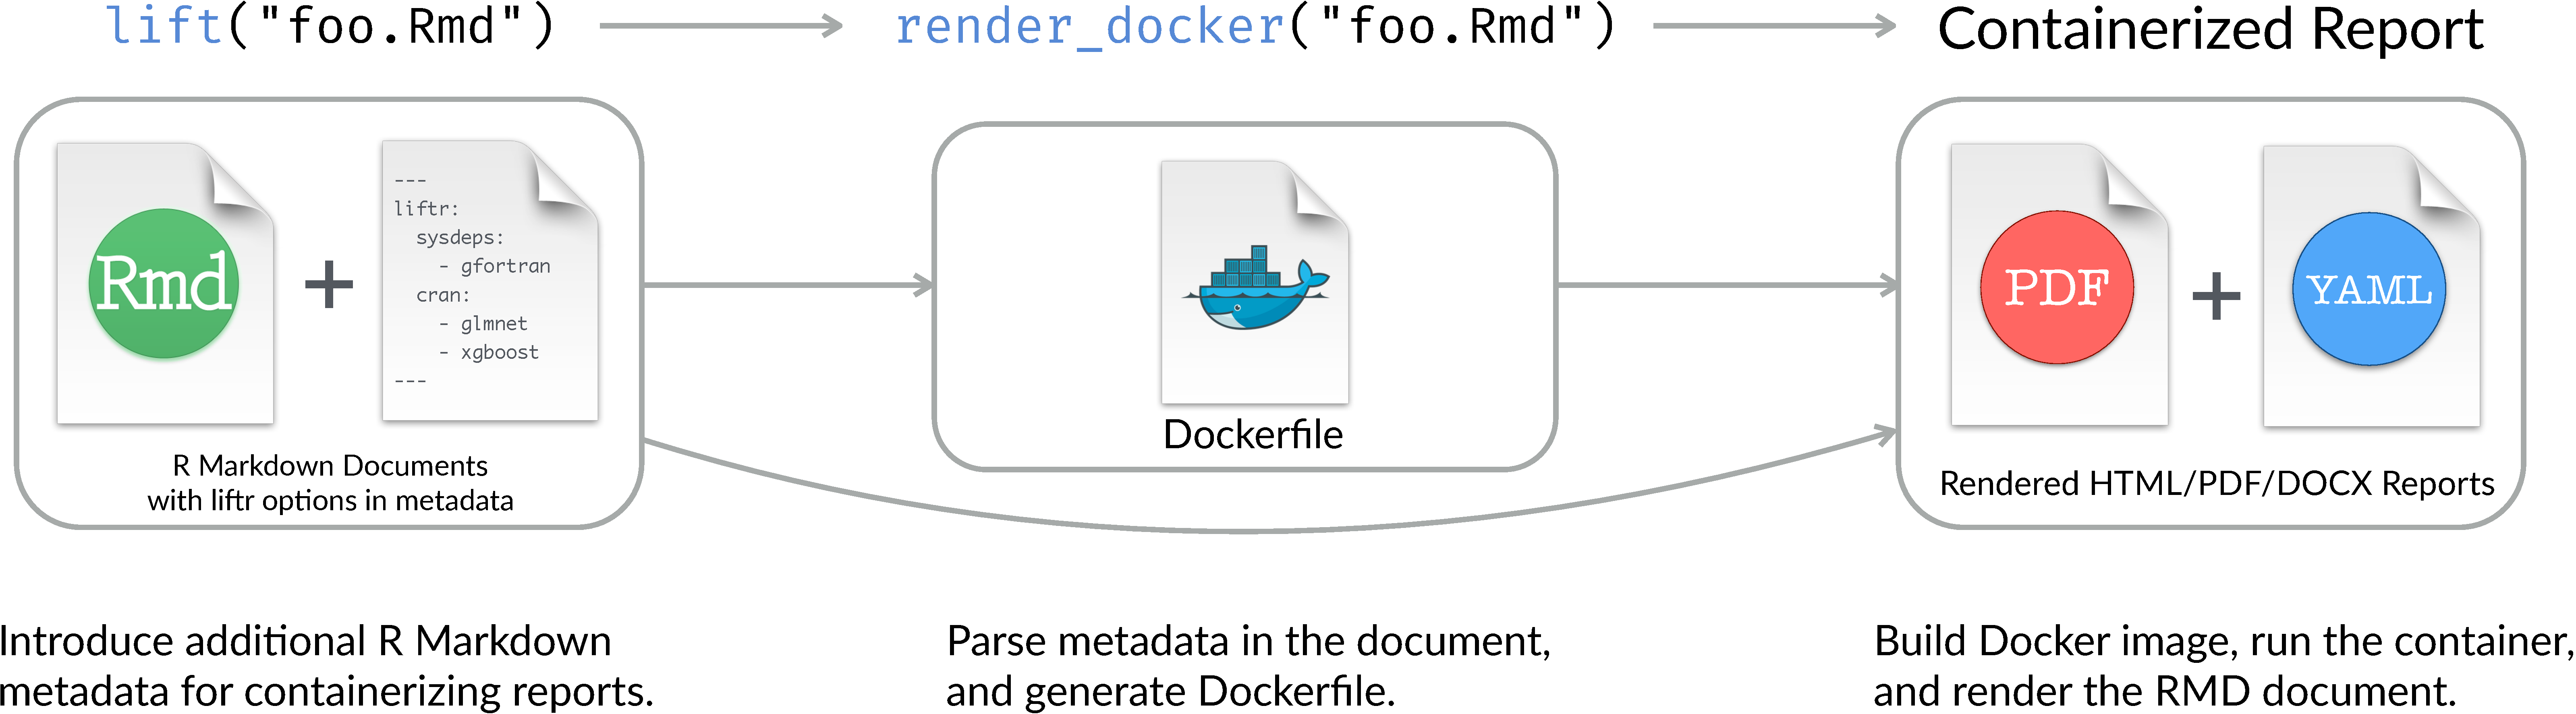
\includegraphics[width=\textwidth]{liftr-workflow}
  \caption{The liftr workflow for rendering containerized R Markdown documents.}
  \label{figure:liftr}
\end{figure}

\emph{knitr} and R Markdown are used as the template engine to generate
the \texttt{Dockerfile}. Features such as caching container layers for
saving image build time, automatic housekeeping for fault-tolerant
builds, and Docker status check are supported by \emph{liftr}. Four
RStudio addins are also offered by \emph{liftr} to allow push-button
compilation of documents and provide better IDE integrations.

Three basic principles are followed to design the \emph{liftr} package
since its inception.

\begin{enumerate}
\def\labelenumi{\arabic{enumi}.}
\item
  Continuous reproducibility. Continuous integration, continuous
  delivery, and continuous deployment are well-accepted practices in
  software engineering. Similarly, it is believed by the authors of
  \emph{liftr} that ensuring computational reproducibility means a
  continuous process instead of creating static data/code archives or a
  one-time deal. Specifically, the software packages used in data
  analysis should be upgraded regularly in a manageable way. Therefore,
  \emph{liftr} supports specifying particular versions of package
  dependencies, while users are encouraged to always use the latest
  version of packages (without a version number) by default.
\item
  Document first. Many data analysis workflows could be wrapped as
  either R packages or dynamic documents. In \emph{liftr}, the endpoint
  of dynamic report creation is the focus of containerization, because
  this offers more possibilities for organizing both computations and
  documentation. Users are encouraged to start thinking from the visible
  research output from the first day.
\item
  Minimal footprint. R Markdown and Docker are already complex software
  systems. Making them work together seamlessly can be complicated.
  Therefore, API designs such as function arguments are simplified while
  being kept as expressive and flexible as possible.
\end{enumerate}

In summary, \emph{liftr} tries to redefine the meaning of computational
reproducibility by offering system-level reproducibility for data
analysis. It provided a practical way for achieving it --- a new
perspective on how reproducible research could be done in reality.
Further, sharing system environments for data analysis also becomes
extremely easy, since users only need to share the R Markdown document
(with a few extra metadata fields), and compile them with \emph{liftr}.
As an example, \emph{liftr} demonstrated its advantage for R
Markdown-based computational workflow orchestration, by effortlessly
containerizing 18 complex \emph{Bioconductor} workflows in the DockFlow
project (\url{https://dockflow.org}) in 2017.

One of the key tool of Docker are \texttt{Dockerfile}s, which can be
thought of as ``recipes'' used to build a specific image. But building
these files can feel like a workflow break as it demands to open a
separate file, and / or to write a small wrapper around R's
\texttt{write()} function to add elements to the file. At the same time,
doing it by hand prevents from using programming language for what they
are good for: iteration, and automation. Iteration and automation for
\texttt{Dockerfile}s is the very reason behind
\href{https://github.com/ColinFay/dockerfiler}{\texttt{dockerfiler}}, an
R package designed for building \texttt{Dockerfile}s straight from R.

For example, the
\textbf{\href{https://github.com/ThinkR-open/golem}{\texttt{golem}}}
package makes an heavy use of \texttt{dockerfiler} when it comes to
creating the \texttt{Dockerfile} for building production-grade Shiny
applications and deploying them. The reason behind this is that
\texttt{dockerfiler}, on top of being scriptable from R, can leverage
all the tools available in R to parse a \texttt{DESCRIPTION} file, to
get system requirements, to list dependencies, versions, etc.

\hypertarget{using-r-to-power-enterprise-software-in-production-environments}{%
\subsection{Using R to power enterprise software in production
environments}\label{using-r-to-power-enterprise-software-in-production-environments}}

\label{enterprise}

R has been historically viewed as a tool for analysis and scientific
research--not for creating software that corporations can rely on to
continously run in real time. However, thanks to advancements in R
running as a web service, along with with the ability to deploy R in
Docker containers, modern enterprises are now capable of having
real-time machine learning powered by R.

The backbone of this work is the \pkg{plumber}
(\url{https://www.rplumber.io/}) package. The plumber package allows R
to be used to host web services through RESTful APIs. When R is running
on a server, a different server can ask R to make a computation through
an HTTP request and get an immediate response. For instance, if a data
scientist at a company creates a machine learning model to tell which
customers are likely to make a repeat purchase, if they serve the model
through a plumber API then someone else on the marketing team could
write software that sends different emails depending on that real-time
prediction. Plumber syntax is simple to read and understand: the API is
created by commenting above function names in an R script.

\begin{verbatim}
#* Return the sum of two numbers
#* @get /random
function(){
  runif()
}
\end{verbatim}

\emph{Example of a plumber API to generated a random number by visiting
\texttt{http://127.0.0.1/random}}

Plumber becomes far more powerful with the addition of Docker. Docker
can be used to create images that
\href{https://www.rplumber.io/docs/hosting.html\#docker}{include both R
and plumber}. Then when the image is deployed, that creates the web
endpoints that other services can hit and call the R code. This pattern
of deploying code mimics those used by software engineering services
created in Java, Python, and other modern languages. By using Docker to
deploy plumber APIs, R can be used alongside those langages as a first
class member of a software engineering technical stack.

At T-Mobile, R is used to power real-time services that are called over
a million times a day. T-Mobile created a set of neural network machine
learning natural language processing models to help customer care agents
manage text-based messages for customers
\citep{t-mobile_enterprise_2018}. The models are convolutional neural
networks that use the RStudio Keras package and are built on top of a
Rocker Docker image. Since the models power tools for agents and
customers, they need to have extremely high uptime and reliability--and
they found that R is able to perform. The AI @ T-Mobile team open
sourced their Docker images
\href{https://github.com/tmobile/r-tensorflow-api}{on GitHub}.

\hypertarget{deployment-to-the-cloud}{%
\subsection{Deployment to the cloud}\label{deployment-to-the-cloud}}

\label{deployment}

The cloud is the natural environment of containers, and is the natural
mechanism to deploy R server applications.

\begin{itemize}
\tightlist
\item
  \texttt{RSelenium}
\item
  \href{https://cloudyr.github.io/googleComputeEngineR/}{\texttt{googleComputeEngineR}}
  (function \texttt{gce\_vm\_template()})

  \begin{itemize}
  \tightlist
  \item
    To enable quick deployments of key R services such as RStudio and
    Shiny onto cloud virtual machines (VMs), this package utilises
    Dockerfiles to move the labour of setting up those services from the
    user to a premade Docker image. For example, by specifying the
    template \texttt{template="rstudio"} in
    \texttt{gce\_vm\_template()/gce\_vm()} an up to date RStudio Service
    image is launched. Specifying \texttt{template="rstudio-gpu"} will
    launch an RStudio Server image with a GPU attached, etc.\\
  \end{itemize}
\item
  \href{https://github.com/sckott/analogsea}{\texttt{analogsea}}
  (digital ocean R client)
\item
  \href{https://www.rplumber.io/docs/hosting.html\#docker}{\texttt{plumber}}
\item
  \href{https://github.com/tmobile/r-tensorflow-api}{production
  deployment of neural networks} \citep[\citet{nolistic}]{jnolis}
\item
  Kubernetes - A popular platform for managing Docker containers is
  \href{https://kubernetes.io/}{Kubernetes}, which is used for a wide
  variety of containerized applications. It may be your organisation has
  a Kubernetes cluster already for other applications. Docker containers
  are used within Kubernetes clusters to hold native code, for which
  Kubernetes creates a framework around network connections and scaling
  of resources up and down. An introduction on using
  \href{https://code.markedmondson.me/r-on-kubernetes-serverless-shiny-r-apis-and-scheduled-scripts/}{Kubernetes
  with R is published at this blog post}.
\item
  \href{https://cran.r-project.org/package=AzureContainers}{\texttt{AzureContainers}}:
  Umbrella package for working with containers in Microsoft's Azure
  cloud. Provides interfaces to three Azure services: Container
  Registry, Container Instances (for running individual containers), and
  Kubernetes Services (for orchestrated deployments)
\end{itemize}

While Plumber provides the low-level infrastructure for turning a
statistical model into a predictive service, for production purposes it
is usually necessary to take into account considerations such as
scalability, reliability and ease of management. A single container is
limited in the volume of requests it can service. Furthermore, if the
container goes down, or is occupied with processing a computationally
intensive task, the service becomes unavailable until it is restarted.

These issues can be mitigated by deploying not a single container, but a
\emph{cluster} of containers, orchestrated as a single deployment. The
deployment system of choice at the time of writing is
\href{https://kubernetes.io}{Kubernetes}. This allows you to deploy a
single image to a pool of servers, which can then serve requests in
parallel. Client-side requests are made to the cluster ingress endpoint,
which then redirects them to individual servers. The orchestrator can
identify cluster nodes that have failed, and restart them automatically;
it can also detect when there is no capacity to service more requests,
and start additional servers and containers as needed.

While these load-balancing and autoscaling properties of a Kubernetes
cluster are invaluable, they are still limited by the hardware resources
that it has access to. A cluster cannot scale out if it has run out of
servers. This issue in turn can be addressed by deploying not to
on-premise servers but to the cloud, where effectively unlimited
computing resources are available (as long as one can pay for them).
From a management perspective, cloud deployments have the additional
advantage that hardware maintenance becomes the responsibility of the
cloud provider, eliminating another pain point. Orchestrator services
are available from all the major cloud service providers, including
Amazon Web Services (AWS), Google Cloud Platform, and Microsoft Azure.

An example of an R package for working with containers in the cloud is
AzureContainers, which interacts with three Azure services: Container
Instances (for running a single container), Container Registry (a
private docker registry service), and Kubernetes Service (for Kubernetes
on Azure). AzureContainers provides a lightweight yet powerful interface
for working with Resource Manager, the framework for deploying and
managing arbitrary resources in Azure. On the client side, it provides
simple shells to the Docker, Kubectl and Helm tools that are commonly
used for managing containers and Kubernetes clusters.

Here is some simple code that pushes a Docker image to an Azure
Container Registry, and then creates a deployment using Azure Kubernetes
Service. This is a slightly modified version of the code from the
``Deploying a prediction service with Plumber'' AzureContainers
vignette. The code makes use of a yaml file to define the deployment and
predictive service, which is standard practice with Kubernetes; the yaml
can be seen in the aforementioned vignette.

\begin{verbatim}
library(AzureContainers)
# create a resource group for our deployments
deployresgrp <- AzureRMR::get_azure_login()$
    get_subscription("subscription_id")$
    create_resource_group("deployresgrp", location="australiaeast")

### create a container registry
deployreg_svc <- deployresgrp$create_acr("deployreg")

# build our image (a random forest on the Boston housing data, available in the MASS package)
call_docker("build -t bos-rf .")

# upload the image to Azure
deployreg <- deployreg_svc$get_docker_registry()
deployreg$push("bos-rf")


### create a Kubernetes cluster with 2 nodes
deployclus_svc <- deployresgrp$create_aks("deployclus", agent_pools=aks_pools("pool1", 2))

# grant the cluster pull access to the registry
gr <- AzureGraph::get_graph_login()
aks_app_id <- deployclus$properties$servicePrincipalProfile$clientID
reg$add_role_assignment(gr$get_app(aks_app_id), "Acrpull")


# get the cluster endpoint
deployclus <- deployclus_svc$get_cluster()

# create and start the service
deployclus$create("bos-rf.yaml")
\end{verbatim}

Once the service has been created, we can check on its status and obtain
predictions:

\begin{verbatim}
deployclus$get("deployment bos-rf")
#> Kubernetes operation: get deployment bos-rf  --kubeconfig=".../kubeconfigxxxx"
#> NAME      DESIRED   CURRENT   UP-TO-DATE   AVAILABLE   AGE
#> bos-rf    1         1         1            1           5m

deployclus$get("service bos-rf-svc")
#> Kubernetes operation: get service bos-rf-svc  --kubeconfig=".../kubeconfigxxxx"
#> NAME         TYPE           CLUSTER-IP   EXTERNAL-IP     PORT(S)          AGE
#> bos-rf-svc   LoadBalancer   10.0.8.189   xxx.xxx.xxx.xxx 8000:32276/TCP   5m 


response <- httr::POST("http://xxx.xxx.xxx.xxx:8000/score",
    body=list(df=MASS::Boston[1:10,]), encode="json")
httr::content(response, simplifyVector=TRUE)
#> [1] 25.9269 22.0636 34.1876 33.7737 34.8081 27.6394 21.8007 22.3577 16.7812 18.9785
\end{verbatim}

Note that Plumber, by itself, provides no authentication or security
features; anybody who knows the cluster's IP address can access the
predictive service. At minimum, a basic authentication layer should be
added to any Kubernetes deployment. Standard Kubernetes procedure
involves creating an ingress controller, for example with the nginx or
traefik reverse proxy software, and one can then add
application-specific authentication layers on top of that (for example,
to authenticate with a user's Azure Active Directory or LDAP
credentials). More details can be found from most Kubernetes learning
resources, and are outside the scope of this paper.

\hypertarget{continuous-integration-and-continuous-delivery-colinfaynoamross-colinfay}{%
\subsection{\texorpdfstring{Continuous integration and continuous
delivery
\citep[\citet{ColinFay}]{noamross}}{Continuous integration and continuous delivery , @ColinFay{[}@noamross, @ColinFay{]}}}\label{continuous-integration-and-continuous-delivery-colinfaynoamross-colinfay}}

\label{cicd}

The controlled nature of containers, i.e., it is possible to define the
software environment very well, even on remote machines, make them also
useful for continuous integration (CI) and continuous delivery of
applications.

\begin{itemize}
\tightlist
\item
  DevOps

  \begin{itemize}
  \tightlist
  \item
    \url{https://www.opencpu.org/posts/opencpu-with-docker/}
  \end{itemize}
\end{itemize}

When doing continuous integration and continuous delivery, it's crucial
to test in an environment that matches the production environment. Tools
like \texttt{Gitlab-CI} are built on top of Docker images: the user
specifies a base Docker image, and the whole tests are run inside this
environment. But, as we just said, this environment has to be fixed, but
it also have to contain the necessary toolkit. In order to achieve that,
\href{https://github.com/ColinFay/r-ci}{\texttt{r-ci}} combines
\texttt{rocker} versioning and a series of tools specifically designed
for testing. That way, package builders can use this image as a base
image for there testing environment, without having to install the
necessary packages every time they need to run a new test.

\begin{itemize}
\tightlist
\item
  \href{https://github.com/dynverse/dynwrap_containers/blob/master/.travis.yml}{dynwrap}
  \citep{rcannood}

  \begin{itemize}
  \tightlist
  \item
    For this project, we use travis-ci to build rocker-derived
    containers, test them, and only push them to docker hub (from
    travis-ci.org) if the integration tests succeed.
  \end{itemize}
\item
  Google Cloud Build

  \begin{itemize}
  \tightlist
  \item
    \url{https://cloud.google.com/cloud-build/}
  \item
    Cloud Build is another continuous intergation service that helps
    move the workload of building the Docker images to an online
    service. Cloud Build can be set up to build the Dockerfiles on each
    GitHub commit or release. This means you do not need to build the
    Docker images locally, which can tie up resources since Docker
    images can be several GBs and take a long time to compile. Google
    Cloud Build works alongside Google Container Registry to allow you
    to build private and public Docker images, which allows you to build
    up your own dependency graphs for downstream applications.
  \item
    \url{https://code.markedmondson.me/googleCloudRunner/articles/cloudbuild.html}
  \end{itemize}
\end{itemize}

\hypertarget{common-or-public-work-environments}{%
\subsection{Common or public work
environments}\label{common-or-public-work-environments}}

\label{workenvs}

The fact that Docker images are portable and well defined make them
useful when more than one person needs access to the same computing
environment. This is even more useful when some of the users do not have
the expertise to create such an environment themselves, and when these
environments can be run in public or shared infrastructure.

\textbf{\pkg{holepunch}} (\url{https://github.com/karthik/holepunch}) is
an R package that was designed to make sharing work environments
accessible to novice R users based on \textbf{Binder}. The
\href{https://mybinder.readthedocs.io/en/latest/}{Binder project},
maintained by the team behind Jupyter, makes it possible for users to
create and share their computing environments with others
\citep{jupyter_binder_2018}. A \emph{BinderHub} allows anyone with
access to a web browser and an internet connection to launch a temporary
instance of these custom environments and execute any workflows
contained within. From a reproducibility standpoint, Binder makes it
exceedingly easy to compile a paper, visualize data, and run small
examples from papers or tutorials without the need for any local
installation. To set up Binder for a project, a user typically starts at
an instance of a BinderHub and passes the location of a repository with
a workspace, e.g., a hosted Git repository, or a data repository like
Zenodo. Binder's core internal tool is
\href{https://repo2docker.readthedocs.io/en/latest/config_files.html}{\texttt{repo2docker}}.
It deterministically builds a Docker image by parsing the contents of a
repository, e.g., project dependency configurations or simple
configuration files. In the most powerful case, \texttt{repo2docker}
builds a given \texttt{Dockerfile}. While this approach works well for
most run of the mill Python projects, it is not so seamless for R
projects. For any R projects that use the Tidyverse suite
\citep{wickham_welcome_2019}, the time and resources required to build
all dependencies from source can often time out before completion,
making it frustrating for the average R user. \texttt{holepunch} removes
some of these limitations by leveraging Rocker images that contain the
Tidyverse along special Jupyter dependencies, and only installs
additional packages from CRAN and Bioconductor that are not already part
of these images. It short cicuits the configuration file parsing in
\texttt{repo2docker} and starts with the Binder/Tidyverse base images,
which eliminates a large part of the build time and in most cases
results in a binder instance launching within a minute.
\texttt{holepunch} as a side effect also creates a \texttt{DESCRIPTION}
file which then turns any project into a research compendium
\citep{marwick_packaging_2018}. The \texttt{Dockerfile} included with
the project can also be used to launch a RStudio server locally, i.e.,
independent of Binder, which is especially useful when more or special
computational resources can be provided there. The local image usage
reduces the number of seperately managed environments and thereby
reduces work and increases portability and reproducibility.

In \textbf{high-performance computing}, one use for containers is to run
workflows on shared local hardware where teams manage their own
high-performance servers. This can follow one of several design
patterns: users may deploy containers to hardware as a work environment
for a specific project, conatiners may provide per-user persistent
environments, or a single container can act as a common multi-user
environment for a server. In all cases, though, the containerized
approach provides several advantages: First, users may use the same
image and thus work environment on desktop and laptop computers, as
well. The former models provide modularity, while the latter approach is
most similar to a simple shared server. Second, software updates can be
achieved by updating and redeploying the container, rather than tracking
local installs on each server. Third, the containerized environment can
be quickly deployed to other hardware, cloud or local, if more resources
are neccessary or in case of server destruction or failure. In any of
these cases, users need a method to interact with the containers, be it
and IDE, or command-like access and tools such as SSH, which is usually
not part of standard container recipes and must be added. The Rocker
project provides containers pre-installed with the RStudio IDE. In cases
where users store nontrivial amounts of data for their projects, data
needs to persist beyond the life of the container. This may be via in
shared disks, attached network volumes, or in separate storage where it
is uploaded between sessions. In the case of shared disks or
network-attached volumes, care must be taken to persist user
permissions, and of course backups are still neccessary. When working
with multiple servers, an automation framework such as
\href{https://www.ansible.com}{Ansible} may be useful for managing
users, permisions, and disks along with containers.

Using \textbf{GPUs} (graphical processing units) as a specialised
hardware from containerized common work environments is also possible
and useful \citep{haydel_enhancing_2015}. GPUs are increasingly popular
for compute-intensive machine learning (ML) tasks, e.g., deep artificial
neural networks \citep{schmidhuber_deep_2015}. Though in this case,
containers are not completely portable between hardware environments,
but the software stack for ML with GPUs is so complex to set up that a
ready-to-use container is helpful. Containers running GPU software
require drivers and libraries specific to GPU models and versions, and
containers require a specialized runtime to connect to the underlying
GPU hardware. For NVIDIA GPUs, the
\href{https://github.com/NVIDIA/nvidia-docker}{NVIDIA Container Toolkit}
includes a specialized runtime plugin for Docker and a set of base
images with appropriate drivers and libraries. The Rocker project
\href{https://github.com/rocker-org/ml}{has a repository} with (beta)
images based on these that include GPU-enabled versions of
machine-learning R packages, e.g., \texttt{rocker/ml} and
\texttt{rocker/tensorflow-gpu}.

\textbf{Teaching} is a further example where sharing a prepared
computing environment can greatly improve the process, especially for
courses that require access to a relatively complex setup of software
tools, e.g., as in the case of database systems. R is a fantastic tool
when it comes to interfacing with databases: almost every open source
and proprietary database system has an R package that allows users to
connect and interact with the it This flexibility is even broader now
that we have tools like \texttt{DBI}, that allows to create a common API
for interfacing these databases, or like \texttt{dbplyr}, which are
designed to run \texttt{dplyr} code straight against the database. But
learning and teaching these tools comes with a cost: the cost of
deploying or having access to an environment with the softwares and
drivers installed. For people teaching R, it can become a barrier if
they need to install local versions of the drivers, or to connect to
remote instances which might or might not be made available by IT
services. Giving access to a sandbox for the most common database
environments is the idea behind
\textbf{\href{https://github.com/ColinFay/r-db}{\texttt{r-db}}}
\citep{ColinFay}, a Docker image that contains everything needed to
connect, from R, to a database. Notably, with \texttt{r-db}, the users
don't have to install complex drivers or to configure their machine in a
specific way. On top of that, \texttt{r-db} comes with a comprehensive
\href{http://colinfay.me/r-db/}{online guide}, explaining how to spin a
Docker instance of a specific database, and how to use \texttt{r-db} to
connect to it. Each package contained inside this image also has a
series examples, so that the user can get started with the database
right away. The \texttt{rocker/tidyverse} base image ensures that users
can also readily use packages for analysis, display, and reporting.

\textbf{\href{https://github.com/att/rcloud/tree/master/docker}{RCloud}}
uses a \texttt{rocker/drd} base image for creation of collaborative data
analysis and visualisation environments.

\hypertarget{using-docker-in-a-commercial-data-science-platform}{%
\subsection{Using Docker in a commercial Data Science
Platform}\label{using-docker-in-a-commercial-data-science-platform}}

\label{rstudio}

In addition to embedding RStudio Open Source Server inside of Docker
images, such as Rocker, RStudio offers the moduler data science platform
\href{https://rstudio.com/products/team/}{RStudio Team}, a commercial
product allowing teams of data scientists and their respective IT/DevOps
groups to develop and deploy code in R and Python. RStudio team enables
these groups to use the benefits of containers, without requiring users
to learn new tools or directly interact with containers. Notable
patterns include:

\begin{enumerate}
\def\labelenumi{\arabic{enumi}.}
\tightlist
\item
  \emph{To deploy and manage RStudio Professional Products:} Many
  RStudio customers are managing professional products in Docker
  containers as an alternative to bare-metals servers or virtual
  machines. Best practices for
  \href{https://support.rstudio.com/hc/en-us/articles/360021594513-Running-RStudio-with-Docker-containers}{running
  RStudio with Docker containers} as well as
  \href{https://github.com/rstudio/rstudio-docker-products}{Docker
  images} for RStudio's commerical products are available.
\item
  \emph{To run interactive RStudio sessions on a cluster:} In the
  RStudio Server Pro 1.2 release in 2019, RStudio added new
  functionality called
  \href{https://solutions.rstudio.com/launcher/overview/}{Launcher}. It
  gives users the ability to spawn R sessions and background jobs in a
  scalable way on external clusters, e.g.,
  \href{https://support.rstudio.com/hc/en-us/articles/360019253393-Using-Docker-images-with-RStudio-Server-Pro-Launcher-and-Kubernetes}{Kubernetes
  based on Docker images} or \href{https://slurm.schedmd.com/}{Slurm}
  clusters, and optionally, with Singularity containers. A key benefit
  of Launcher is the ability for R and Python users to interactively
  work in RStudio without learning about Docker at all - while still
  leveraging containers and Kubernetes. Users can submit batch jobs to
  Kubernetes clusters without writing specific deployment scripts.
\end{enumerate}

\href{https://rstudio.com/products/connect/}{RStudio Connect} is a
commercial publishing platform to deploy dashboards, REST APIs, and
other R and Python content into production. RStudio Connect uses an
approach to isolate deployed R applications that is similar to Docker's
filesystem and process namespacing and leverages the
\href{https://rstudio.com/products/package-manager/}{RStudio Package
Manager} to manage R environments including system dependencies. RStudio
Package manager may also be used to
\href{https://environments.rstudio.com/docker}{manage their R
environments and package versions with Docker} and to ensure
deterministic image builds.

\hypertarget{processing-div}{%
\subsection{Processing {[}div{]}}\label{processing-div}}

\label{processing}

The portability of containers becomes particularly useful when complex
processing tasks shall be offloaded to a server.

\begin{itemize}
\tightlist
\item
  Docker images for cloud services

  \begin{itemize}
  \tightlist
  \item
    A popular application of using Docker is to create the environments
    that can run in parallel for speeding up R code. For example,
    \href{https://CRAN.R-project.org/package=googleComputeEngineR}{\texttt{googleComputeEngineR}}'s
    \texttt{gce\_vm\_cluster()} function can create clusters of 2 or
    more virtual machines, running multi-CPU architectures. Instead of
    running a local R script with the local CPU and RAM restrictions,
    the same code can be processed on all CPU threads of the cluster of
    machines in the cloud, all running in a Docker container with the
    same R environments. This is achieved through
    \texttt{googleComputeEngineR}'s integration with the R parralisation
    library
    \href{https://CRAN.R-project.org/package=future}{\texttt{library(future)}
    by Henrik Bengtsson}. Local R computation can be thrown up to a
    multi-CPU and VM environment to achieve parrell computation in a few
    lines of R code in your local session. -
    \href{https://cloudyr.github.io/googleComputeEngineR/articles/massive-parallel.html}{some
    demonstrations are available here}.
  \end{itemize}
\item
  \href{https://cloud.run}{Google Cloud Run} - This is a CaaS
  (Containers as a Service) that lets you launch a Docker container
  without worrying about underlying infrastructure. This dispenses with
  the developer creating a cloud server to run the Docker image on, by
  abstracting away those servers to a more serverless configuration.
  Cloud Run lets you run your code on top of a managed or your own
  Kubernetes cluster running Knative, and can accept any Docker image.
  The service takes care of network ingress, scaling machines up and
  down to zero, authentication and authorisation, all features which are
  non-trivial for a developer to create on their own. This can be used
  to scale up R code to millions of instances if they need to, with
  little or no changes to existing code. An R implementation is shown
  here at
  \href{https://github.com/MarkEdmondson1234/cloudRunR}{cloudRunR} which
  uses Cloud Run to create a scalable R plumber API.

  \begin{itemize}
  \tightlist
  \item
    How does this relate to
    \url{https://code.markedmondson.me/googleCloudRunner/index.html} ?`
  \end{itemize}
\item
  \texttt{batchtools} \citep{Lang2017batchtools} can
  \href{https://mllg.github.io/batchtools/reference/makeClusterFunctionsDocker.html}{schedule
  jobs with Docker Swarm}
\item
  scalable deployments, e.g., start with numerous Shiny talks mentioning
  Rocker at useR!2017
\item
  \href{https://github.com/dynverse/dynmethods}{dynmethods}
  \citep{rcannood}: In order to evaluate ±50 computational methods which
  all used different environments (R, Python, C++, \ldots{}), we wrapped
  each of them in a docker container and can execute these methods from
  R. Again, all of these containers are being built on travis-ci, and
  will only be pushed to docker hub if the integration test succeeds.
\item
  \pkg{drake},
  \url{https://docs.ropensci.org/drake/index.html?q=docker\#with-docker}
\end{itemize}

\hypertarget{packaging-programs-for-processing-pipelines}{%
\subsection{Packaging programs for processing
pipelines}\label{packaging-programs-for-processing-pipelines}}

\label{packaging}

Docker is perfectly suited to package and execute any software and data,
and is a good candidate to build complex processing pipelines
independent of the used programming language. Because of the original
use case (see~\nameref{introduction}), Docker does not have a standard
mechanism to chain a number of containers together, i.e., to define how
environment variables, volume mounts, or ports can be used to pass input
parameters and data into a container and how to get results out. Some
packages, e.g.~\pkg{containerit}, provide a Docker image that can be
used similar as a CLI, but the usage is
cumbersome\footnote{\href{https://o2r.info/containerit/articles/container.html}{https://o2r.info/containerit/articles/container.html}}.

\textbf{\pkg{outsider}} (\url{https://antonellilab.github.io/outsider/})
tackles the problem of integrating external programmes into an R
workflow \citep{bennett_outsider_2019}. Installation and usage of
external programmes can be cumbersome and even prohibited if platform
dependent. Therefore \pkg{outsider} uses the platform-independent Docker
images to encapsulate processes in \emph{outsider modules}. Each
outsider modules has a \texttt{Dockerfile} and an R package with
functions for interacting with the encapsulated tool. A user only needs
to use the given functions to install a module and can then integrate a
tool into their own workflow seaminglessly using only R functions. The
module takes care of transmitting arguments and sending and receiving
files to and from a container. Outsider modules are hosted, e.g., on
GitHub, and \pkg{outsider} contains discovery functions for them.

\hypertarget{research-compendia}{%
\subsection{Research Compendia}\label{research-compendia}}

\label{compendia}

\begin{itemize}
\tightlist
\item
  researchcompendia.science
\item
  \url{https://github.com/benmarwick/rrtools}
\item
  \pkg{renv}, \url{https://rstudio.github.io/renv/articles/docker.html}
\item
  what to copy in and what not
\end{itemize}

\hypertarget{development-and-debugging}{%
\subsection{Development and debugging}\label{development-and-debugging}}

\label{development}

Containers can also serve as useful playgrounds to create environments
ad-hoc or to provide very specific environments that are not needed or
not easily available in day-to-day development. These environments may
have specific versions of R, of R extension packages, and of system
libraries used by R extension packages, and all of the above in a
specific combination.

First, such containers can greatly facilitate \textbf{fixing bugs},
because developers can readily start and later discard a container to
investigate a bug report without affecting their regular system, and
potentially having to revert changes back. Using the Rocker images with
RStudio, these disposable environments lack no development comfort
(cf.~Section~\nameref{compendia}). \citet{eddelbuettel_debugging_2019}
describes an example how a Docker container was used to debug an issue
with a package only occuring with a particular version of Fortran, and
using tools which are not readily available on all platforms (e.g., not
on macOS). For the \href{https://www.r-spatial.org/}{R-spatial
community}, using containers is particularly useful, because of the
strong integration of system libraries in core packages for geospatial
data modelling and analysis. Purpose built Docker are used to prepare
for upcoming releases of system libraries, individual bug reports, and
for the lowest supported versions of system libraries
\textbackslash{}footnote\{\href{https://github.com/r-spatial/sf/tree/master/inst/docker}{https://github.com/r-spatial/sf/tree/master/inst/docker},
\textbackslash{}href\{\url{https://github.com/Nowosad/rspatial_proj6}\}\{\url{https://github.com/Nowosad/rspatial_proj6}\},
\href{https://github.com/r-spatial/sf/issues/1231#issuecomment-570076440}{https://github.com/r-spatial/sf/issues/1231\#issuecomment-570076440}\}.

There are also special images for identifying problems beyond the mere R
code, such as \textbf{debugging R memory problems}. The images
significantly reduce the barrier to follow complex steps for fixing
memory allocation bugs \citep[cf. Section~4.3 in][]{core_writing_1999}.
These problems are hard to debug and critical, both because when they
occur they lead to fatal crashing processes.
\href{https://github.com/rocker-org/r-devel-san}{\texttt{rocker/r-devel-san}}
and
\href{https://github.com/rocker-org/r-devel-san-clang}{\texttt{rocker/r-devel-ubsan-clang}}
are Docker images have a particularly configured version of R to trace
such problems with gcc and clang compilers, respectively
\citep[cf.~\pkg{sanitizers} for examples,][]{eddelbuettel_sanitizers_2014}.
The image \href{https://github.com/wch/r-debug}{\texttt{wch/r-debug}} is
a purpose built Docker image with \emph{multiple} instrumented builds of
R, each with a different diagnostic utility activated.

Second, containers are useful for \textbf{testing} R code during
development. To submit a package to CRAN, an R package must work with
the development version of R, which must be compiled locally. That can
be a challenge for some users. The R-hub service (see
Section~\nameref{rhub}) makes it easy to ensure that no errors occur,
but to fix errors a local setup is still often warranted, e.g.~using the
image \texttt{rocker/r-devel}, and to test packages with native code,
which can make the process more complex
\citep[cf.][]{eckert_building_2018}. The R-hub Docker images can also be
used to debug problems locally using various combinations of Linux
platforms, R versions, and
compilers\footnote{See \href{https://r-hub.github.io/rhub/articles/local-debugging.html}{https://r-hub.github.io/rhub/articles/local-debugging.html} and \href{https://blog.r-hub.io/2019/04/25/r-devel-linux-x86-64-debian-clang/}{https://blog.r-hub.io/2019/04/25/r-devel-linux-x86-64-debian-clang/}}.
The images go beyond the configurations, or \emph{flavours}, used by
CRAN for checking
packages\footnote{\href{https://cran.r-project.org/web/checks/check_flavors.html}{https://cran.r-project.org/web/checks/check\_flavors.html}},
e.g., with CentOS-based images, but lack a container for checking on
Windows or OS X. The images greatly support package developers to
provide support on operating systems they are not familiar. The package
\pkg{dockertest} (\url{https://github.com/traitecoevo/dockertest/}) is a
proof of concept for automatically generating \texttt{Dockerfile}s and
building images specifically to run
tests\footnote{\pkg{dockertest} is not actively maintained, but mentioned still because of its interesting approach.}.
These images are accompanied with a special launch script so the tested
source code is not stored in the image but the currently checked in
version from a local Git repository is cloned into the container at
runtime. This approach clearly seperates test environment, test code,
and current working copy of the code.

Third, Docker images can be used \textbf{on CI platforms} to streamline
the testing of packages. \citet{ye_docker_2019} describes how they speed
up the process of testing by running tasks on
\href{https://travis-ci.org/}{Travis~CI} within a container using
\texttt{docker\ exec}, e.g., the package check or rendering of
documentation. \citet{cardozo_faster_2018}, also on Travis~CI saved time
by re-using the testing image as the base iamge for an image intended
for publication on Docker Hub. Especially for long running tests or
complex system dependencies, these approaches seems to improve the
development. Not due to a concern about time, but to control the
environment used on a CI server, even this manuscript was rendered into
a PDF and deployed to a GitHub-hosted website (see \texttt{.travis.yml}
and \texttt{Dockerfile} in the manuscript repository). This gives on the
one hand easy access after every update of the R Markdown source code,
and on the other hand a second controlled environment making sure that
the article renders successfully and correctly.

\hypertarget{conclusions}{%
\section{Conclusions}\label{conclusions}}

This article is a snapshot of the R-corner in a universe of applications
built many-faced piece of software, Docker. \texttt{Dockerfile}s and
Docker images are the go-to methods for collaboration between roles in
an organisation, such as development and IT operations teams, and
between parties in the communication of knowledge, such as research
workflows or education. Docker became synonymous with applying the
concept of containerisation to solve challenges of reproducible
environments, e.g., in research and in development \& production, and of
scalable deployments with the ability to move processing between
machines easily (e.g., locally, one cloud providers VM, another cloud
provider's Container-as-a-Service). Collaboration, reproducibility, and
portability are the common themes behind R packages, use cases, and
applications in this work.

The R packages and use cases presented show the positive drive in the
community to innovate, but also the challenge of keeping up with a
continuously evolving landscape. The use cases contributed by co-authors
also have a degree of overlap. A common language and understanding of
good practices is still taking shape. The easiness with which one can
create a complex software systems, such as an independent Docker image
stack, to serve one's specific needs currently leads to some
fragmentation. It is unclear if Docker alone as a core technology is
really a feasible level of collaboration and abstraction. Furthermore
fragmentation may not be a bad sign but instead a reflection of a
growing market, which is able to sustain multiple related efforts. With
the maturing of core building blocks, such as the Rocker suite of
images, more systems will be built successfully but will also be behind
the curtains.

However, at least \emph{on the level of R packages}, some consolidation
seems in order, e.g., to reduce the number of packages creating
\texttt{Dockerfile}s from R code or controlling the Docker daemon with R
code. It remains to be seen which approach to control Docker, via the
Docker API as \texttt{stevedore} or via system calls as
\texttt{dockyard}/\texttt{docker}/\texttt{dockr}, is more sustainable,
or if the question will be answered by the endurance of maintainers and
sufficient funding. Similarly, the capturing of environments and their
serialization in form of a \texttt{Dockerfile} currently happens at
different levels of abstraction and re-use of functionality seems
reasonable, e.g.~\texttt{liftr} could generate the environment with
\texttt{containerit}, which in turn may use \texttt{dockerfiler} for low
level objects representing a \texttt{Dockerfile}. In this consolidation,
the Rocker Project could play the role of a unifying and coordinating
entity in the future. Though for the moment, the sign of the times
points to more experimentation and feature growth, e.g.~images for
GPU-based computing and artificial intelligence. Even with coding being
more and more accepted as a required, and achievable skill, an easier
access, for example by exposing containerisation benefits via simple
user interfaces in the users' IDE, could be an important next step.
Currently containerisation happens more in the background at the system
level.

New features, which make complex workflows accessible and reproducible,
and variety in packages, even when they have overlapping features, are a
signal and a support for a growing user base. This growth is possibly
the the most important goal for the foreseeable future in the
\emph{Rockerverse}. The dominant position of Docker is a blessing and a
curse for these goals. It could be wise to start experimenting with
non-Docker containerisation tools now, e.g.~R packages interfacing with
other container engines such as
\href{https://github.com/containers/libpod}{podman/buildah} or
\href{https://coreos.com/rkt/}{rkt}, or an R package for creating
Singularity image recipe files. Such efforts help to avoid lock-in and
to design sustainable workflows based on concepts of
\emph{containerisation}, not on their implementation in Docker. If
adoption of containerisation and R continue to grow, the missing pieces
for a success predominantly lie in (a) coordination and documentation of
activities to reduce repeated work in favour of open collaboration, (b)
the sharing of lessons learned from use cases to build common knowledge
and language, and (c) a sustainable continuation and funding for all of
development, community support, and education. A concrete effort to work
towards these pieces is to sustain the structure and captured status quo
from this work in form of a CRAN Task View on containerization.

\hypertarget{author-contributions}{%
\section{Author contributions}\label{author-contributions}}

DN conceived of the presented idea and
\href{https://github.com/nuest/rockerverse-paper/issues/3}{initialised the formation of the writing team},
wrote sections not mentioned below, and revised the full first draft. CB
.. RC and EH wrote the section on interfaces for Docker in R. DE wrote
the introduction and section about Rocker. ME .. CF wrote the paragraphs
about \texttt{r-online}, \texttt{dockerfiler}, \texttt{r-ci} and
\texttt{r-db}. BW .. KR .. NR .. NX wrote the section on liftr. LS \& NT
wrote the section on Bioconductor. All authors approved the final
version.

This articles was collaboratively written at
\href{https://github.com/nuest/rockerverse-paper/}{https://github.com/nuest/rockerverse-paper/}.
The
\href{https://github.com/nuest/rockerverse-paper/graphs/contributors}{contributors page},
\href{https://github.com/nuest/rockerverse-paper/commits/master}{commit history},
and
\href{https://github.com/nuest/rockerverse-paper/issues/}{discussion issues}
provide a detailed view on the respective contributions.

\hypertarget{acknowledgements}{%
\section{Acknowledgements}\label{acknowledgements}}

DN is supported by the project Opening Reproducible Research
(\href{https://www.uni-muenster.de/forschungaz/project/12343}{o2r})
funded by the German Research Foundation (DFG) under project number
\href{https://gepris.dfg.de/gepris/projekt/415851837}{PE~1632/17-1}. The
funders had no role in data collection and analysis, decision to
publish, or preparation of the manuscript.

\bibliography{RJreferences}


\address{%
Daniel Nüst\\
University of Münster\\
Institute for Geoinformatics\\ Heisenbergstr. 2\\ 48149 Münster, Germany\\ \orcid{0000-0002-0024-5046}\\
}
\href{mailto:daniel.nuest@uni-muenster.de}{\nolinkurl{daniel.nuest@uni-muenster.de}}

\address{%
Robrecht Cannoodt\\
Ghent University\\
Data Mining and Modelling for Biomedicine group\\ VIB Center for Inflammation Research\\ Technologiepark 71\\ 9052 Ghent, Belgium\\ \orcid{0000-0003-3641-729X}\\
}
\href{mailto:robrecht@cannoodt.dev}{\nolinkurl{robrecht@cannoodt.dev}}

\address{%
Dirk Eddelbuettel\\
University of Illinois at Urbana-Champaign\\
Department of Statistics\\ Illini Hall, 725 S Wright St\\ Champaign, IL 61820, USA\\ \orcid{0000-0001-6419-907X}\\
}
\href{mailto:dirkd@eddelbuettel.com}{\nolinkurl{dirkd@eddelbuettel.com}}

\address{%
Mark Edmondson\\
IIH Nordic A/S, Google Developer Expert for GCP\\
\\
}
\href{mailto:mark@markedmondson.me}{\nolinkurl{mark@markedmondson.me}}

\address{%
Colin Fay\\
ThinkR\\
5O rue Arthur Rimbaud\\ 93300 Aubervilliers, France\\ \orcid{0000-0001-7343-1846}\\
}
\href{mailto:contact@colinfay.me}{\nolinkurl{contact@colinfay.me}}

\address{%
Karthik Ram\\
Berkeley Institute for Data Science\\
University of California\\ Berkeley, CA 94720, USA\\ \orcid{0000-0002-0233-1757}\\
}
\href{mailto:karthik.ram@berkeley.edu}{\nolinkurl{karthik.ram@berkeley.edu}}

\address{%
Noam Ross\\
EcoHealth Alliance\\
460 W 34th St., Ste. 1701\\ New York, NY 10001, USA\\ \orcid{0000-0002-0233-1757}\\
}
\href{mailto:ross@ecohealthalliance.org}{\nolinkurl{ross@ecohealthalliance.org}}

\address{%
Nan Xiao\\
Seven Bridges Genomics\\
529 Main St, Suite 6610\\ Charlestown, MA 02129, USA\\ \orcid{0000-0002-0250-5673}\\
}
\href{mailto:me@nanx.me}{\nolinkurl{me@nanx.me}}

\address{%
Lori Shepherd\\
Roswell Park Comprehensive Cancer Center\\
Elm \& Carlton Streets\\ Buffalo, New York, 14263, USA\\ \orcid{0000-0002-5910-4010}\\
}
\href{mailto:lori.shepherd@roswellpark.org}{\nolinkurl{lori.shepherd@roswellpark.org}}

\address{%
Nitesh Turaga\\
Roswell Park Comprehensive Cancer Center\\
Elm \& Carlton Streets\\ Buffalo, New York, 14263, USA\\ \orcid{0000-0002-0224-9817}\\
}
\href{mailto:nitesh.turaga@roswellpark.org}{\nolinkurl{nitesh.turaga@roswellpark.org}}

\address{%
Jacqueline Nolis\\
Nolis, LLC\\
Seattle, WA, USA\\ \orcid{0000-0001-9354-6501}\\
}
\href{mailto:jacqueline@nolisllc.com}{\nolinkurl{jacqueline@nolisllc.com}}

\address{%
Heather Nolis\\
T-Mobile\\
12920 Se 38th St.\\ Bellevue, WA, 98006\\
}
\href{mailto:heather.wensler1@t-mobile.com}{\nolinkurl{heather.wensler1@t-mobile.com}}

\address{%
Hong Ooi\\
Microsoft\\
Level 5, 4 Freshwater Place\\ Southbank, VIC 3006, Australia\\
}
\href{mailto:hongooi@microsoft.com}{\nolinkurl{hongooi@microsoft.com}}

\address{%
Ellis Hughes\\
Fred Hutchinson Cancer Research Center\\
Vaccine and Infectious Disease\\ 1100 Fairview Ave. N., P.O. Box 19024\\ Seattle, WA 98109-1024, USA\\
}
\href{mailto:ehhughes@fredhutch.org}{\nolinkurl{ehhughes@fredhutch.org}}

\address{%
Sean Lopp\\
RStudio, Inc\\
RStudio\\ 250 Northern Ave\\ Boston, MA 02210\\
}
\href{mailto:sean@rstudio.com}{\nolinkurl{sean@rstudio.com}}

\address{%
Ben Marwick\\
\\
\\
}


